\section{Analytical applications}

This section collects analytical variational models. Each example begins with a physical or geometric quantity that is additive over small pieces of a curve or surface; integrating those pieces produces the functional to be made stationary. Numerical discretization and numerical optimization are intentionally outside the scope of this chapter.

\subsection{Brachistochrone}
A frictionless particle starts from rest and moves under gravity along a curve $y=u(x)$. The fastest path is not generally the shortest path: a steep initial descent gains speed early, trading distance against travel time. Conservation of energy gives the speed at height $u$ as
\begin{equation}
v=\sqrt{2g(y_0-u)}.
\end{equation}
Since $\mathrm{d}s=\sqrt{1+u'^2}\,\mathrm{d}x$ and $\mathrm{d}t=\mathrm{d}s/v$, the travel time is the functional
\begin{equation}
T[u]=\int_{x_0}^{x_1}
\frac{\sqrt{1+u'^2}}{\sqrt{2g(y_0-u)}}\,\mathrm{d}x.
\end{equation}
\begin{figure}[H]
	\centering
	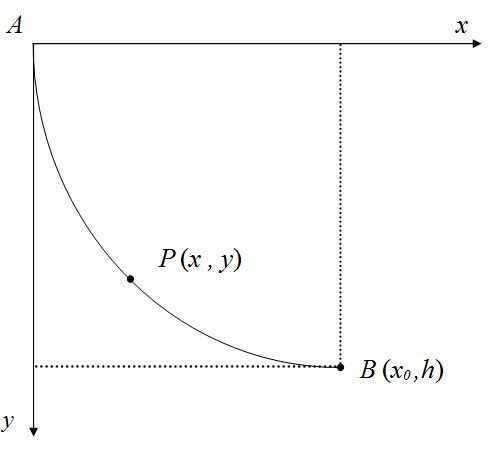
\includegraphics[width=0.46\textwidth]{figures/fastest_track.png}
	\caption{Coordinate setup for the brachistochrone problem.}
	\label{fig:ch03-brachistochrone}
\end{figure}
The physical track is obtained by applying the Euler--Lagrange equation to this integrand. Its solution is a cycloid, not a straight line. The example makes clear that the quantity to optimize must come from the governing physics: minimizing length would answer a different question.

\subsection{Catenary}
For a uniform flexible chain with linear density $\rho$, the gravitational potential energy is
\begin{equation}
U[u]=\rho g\int_{-L/2}^{L/2}u(x)\sqrt{1+u'(x)^2}\,\mathrm{d}x.
\end{equation}
\begin{figure}[H]
	\centering
	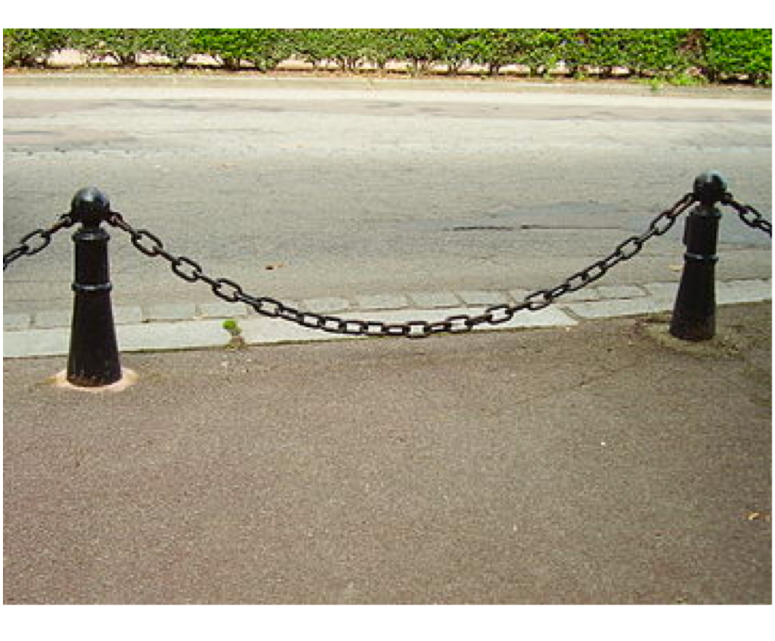
\includegraphics[width=0.42\textwidth]{figures/roadside.png}
	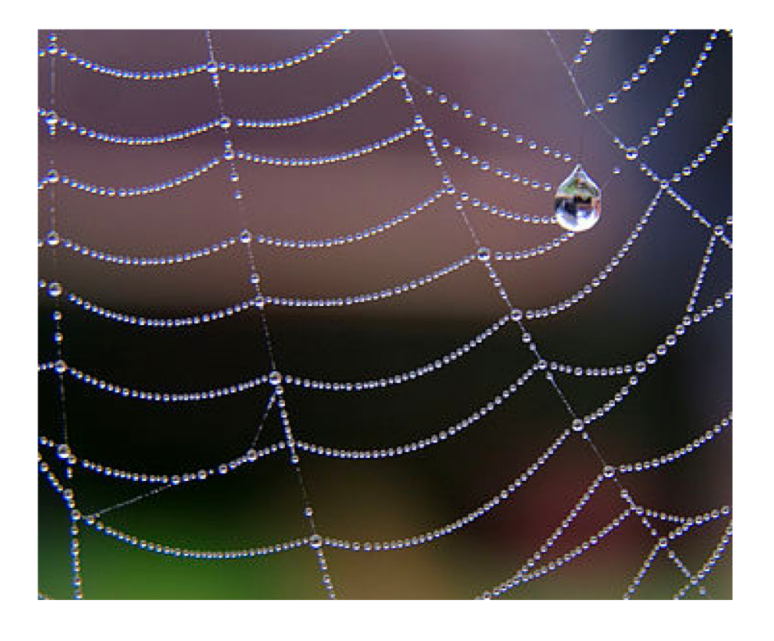
\includegraphics[width=0.42\textwidth]{figures/cobweb.png}
	\caption{Physical examples of catenary-like curves.}
	\label{fig:ch03-catenary-examples}
\end{figure}
For a small segment, $\mathrm{d}m=\rho\,\mathrm{d}s=\rho\sqrt{1+u'^2}\,\mathrm{d}x$, so its potential-energy contribution is $g u\,\mathrm{d}m$. Summing all segments gives the displayed functional. The equilibrium shape minimizes it subject to the endpoint conditions and, when the total chain length is prescribed, an additional length constraint. Solving its Euler--Lagrange equation gives the catenary form
\begin{equation}
u(x)=a\cosh\left(\frac{x-x_c}{a}\right)+u_c,
\end{equation}
with constants determined by the support geometry and chain length. A catenary is therefore a balance of gravity and tension, rather than a parabola; its near-vertex parabolic approximation can nevertheless be useful over a short span.

\subsection{Soap film and minimal surfaces}
For a graph $z=u(x,y)$, the area of a soap film is
\begin{equation}
E[u]=\iint_S\sqrt{1+u_x^2+u_y^2}\,\mathrm{d}x\,\mathrm{d}y.
\end{equation}
A small projected element $\mathrm{d}x\,\mathrm{d}y$ is stretched by the factor $\sqrt{1+u_x^2+u_y^2}$ when lifted to the graph. Since surface tension is proportional to area, an ideal soap film with a fixed boundary makes this area stationary. The field Euler--Lagrange equation is the minimal-surface equation
\begin{equation}
\frac{\partial}{\partial x}
\left(\frac{u_x}{\sqrt{1+u_x^2+u_y^2}}\right)
+\frac{\partial}{\partial y}
\left(\frac{u_y}{\sqrt{1+u_x^2+u_y^2}}\right)=0.
\end{equation}
This equation expresses the vanishing of the mean curvature of the equilibrium surface. Unlike the curve problems, the unknown is now a function of two independent variables, so the variational condition is a partial differential equation.

\subsection{Stationary phase and group velocity}

A wave disturbance in a field $u(x,t)$ can be written as a superposition of plane waves,
\begin{equation}
u(x,t)=\frac{1}{(2\pi)^2}\iint e^{\mathrm{i}(kx-\omega t)}\,\widetilde u(k,\omega)\,\mathrm{d}k\,\mathrm{d}\omega,
\end{equation}
restricted to those $(k,\omega)$ that satisfy the dispersion relation $D(k,\omega)=0$ of the medium. For waves of fixed frequency $\omega$ the relation $\omega=\omega(k)$ singles out the allowed wavenumbers, and the disturbance propagates as
\begin{equation}
u(x,t)=\frac{1}{2\pi}\int e^{\mathrm{i}(kx-\omega(k)t)}\,\widetilde u(k)\,\mathrm{d}k.
\end{equation}

The phase of the integrand, $\phi(k)=kx-\omega(k)t$, oscillates rapidly for generic $k$ and contributions from different wavenumbers interfere destructively. The integrand is appreciable only where $\phi$ is stationary, i.e. where $\phi'(k)=0$. This condition is a constrained stationarity problem: minimize $\phi(k)$ subject to the dispersion relation $D(k,\omega)=0$. The corresponding Lagrange-multiplier equations,
\begin{equation}
x-\lambda\,\frac{\partial D}{\partial k}=0,
\qquad
-t-\lambda\,\frac{\partial D}{\partial \omega}=0,
\end{equation}
combine to give
\begin{equation}
\frac{x}{t}=\frac{\partial\omega}{\partial k}=v_g.
\end{equation}

The dominant contribution therefore travels at the \emph{group velocity} $v_g=\partial\omega/\partial k$, the slope of the dispersion curve at the stationary phase point. This is the physical interpretation of the stationary-phase idea: a wave packet is localized near the point in $(k,\omega)$ space where the phase is stationary, and that point moves through the medium at the group velocity.

\begin{example}[Sound waves]
For a sound wave the frequency and wavenumber satisfy $\omega^2=c^2k^2$ for some constant $c>0$. The group velocity is therefore $v_g=\partial\omega/\partial k=ck$, which equals the phase velocity $c$ here. Sound therefore propagates without dispersion, and a sharp pulse retains its shape as it moves.
\end{example}

\begin{example}[Deep-water gravity waves]
A deep-water surface wave has the dispersion relation $\omega^2=gk$, where $g$ is the acceleration due to gravity. The group velocity is
\begin{equation}
v_g=\frac{\partial\omega}{\partial k}=\frac12\sqrt{\frac{g}{k}},
\end{equation}
which is half the phase velocity $v_p=\omega/k=\sqrt{g/k}$. A wave packet therefore moves at half the speed of its crests: an individual crest travels to the front of the packet and disappears, while new crests form at the back. This is the same phenomenon one observes in a wind-driven swell where sets of crests of similar wavelength outrun the broader pulse.
\end{example}

\subsection{Probabilities from constrained entropy}

A particularly elegant use of Lagrange multipliers arises in the foundations of statistical mechanics. Suppose a random variable $X$ takes the values $x_1,\ldots,x_N$ with probabilities $p_1,\ldots,p_N$. Given only the partial information encoded in a set of average values $\langle X\rangle,\langle Y\rangle,\ldots$, what probabilities should one choose? The maximum-entropy principle selects the $p_i$ that maximize the Shannon entropy
\begin{equation}
S=-\sum_{i=1}^N p_i\ln p_i,
\end{equation}
subject to the normalization constraint $\sum_i p_i=1$ and to whatever further constraints $\sum_i p_i\,\mathcal O_i(x_i)=\langle\mathcal O\rangle$ encode the given averages.

The augmented function reads
\begin{equation}
\mathcal F=-\sum_i p_i\ln p_i-\lambda_0\!\left(\sum_i p_i-1\right)-\sum_a\lambda_a\!\left(\sum_i p_i\,\mathcal O_a(x_i)-\langle\mathcal O_a\rangle\right).
\end{equation}
Varying with respect to $p_i$ yields
\begin{equation}
-\ln p_i-1-\lambda_0-\lambda_a\mathcal O_a(x_i)=0,
\end{equation}
so that
\begin{equation}
p_i=\frac{1}{Z}\exp\!\left(-\sum_a\lambda_a\mathcal O_a(x_i)\right),
\qquad
Z=\sum_i\exp\!\left(-\sum_a\lambda_a\mathcal O_a(x_i)\right).
\end{equation}
The normalization constant $Z$, called the partition function, is determined by the constraint $\sum_i p_i=1$, while the multipliers $\lambda_a$ are fixed by the average-value constraints $\langle\mathcal O_a\rangle$.

\begin{example}[Canonical ensemble]
If the only constraint besides normalization is the average energy $\langle E\rangle$, the maximum-entropy distribution is
\begin{equation}
p_i=\frac{e^{-\beta E_i}}{Z},
\qquad
Z=\sum_i e^{-\beta E_i},
\end{equation}
with the inverse-temperature multiplier $\beta$ determined implicitly by
\begin{equation}
\langle E\rangle=-\frac{\partial\ln Z}{\partial\beta}.
\end{equation}
This is precisely the Boltzmann distribution of equilibrium statistical mechanics; the entropy-maximization principle thus explains why this distribution arises from partial information rather than from dynamics. The derivation is exact, and it carries over to systems with additional conserved quantities such as particle number, in which case a chemical-potential multiplier $\beta\mu$ appears alongside $\beta$.
\end{example}

The same construction produces the Gaussian distribution when one constrains the mean and variance of a continuous variable, the Bose--Einstein and Fermi--Dirac distributions when particle statistics are imposed, and the maximum-entropy image reconstructions used in observational astronomy. In every case the variational principle selects a unique distribution from a set of admissible candidates; the multipliers $\lambda_a$ are the parameters one tunes to match the available data.